\documentclass{article}
\usepackage{graphicx} % Required for inserting images
\usepackage{float}
\usepackage[T1]{fontenc}
\usepackage{amsmath}
\usepackage[margin=1in]{geometry}
\usepackage{booktabs}
\usepackage{tabularx}
\usepackage[hidelinks]{hyperref}

\title{Combining short-only with a 10-share hedge band on the SPY gamma book}
\author{Experiment report \textperiodcentered{} L/S Gamma Desk, QUANTT}
\date{2026-10-16}

\begin{document}

\maketitle

\textbf{Question:} Two rules each passed on their own on 2014-2024: short-only entries and a 10-share hedge band. Does the combination beat short-only alone on net P\&L at 1x and 2x spreads, in both halves, without a worse daily tail?

\textbf{Method:}

\begin{itemize}

\item \textbf{Pre-registration:} the hypothesis card was committed before any run (commit c2f7109).

\item \textbf{Data:} the live paper rules (\texttt{configs/\allowbreak{}paper.\allowbreak{}toml}) are replayed on R2 replay snapshots v1 (config\_hash b040760187f0) over the development window 2014-06-02 to 2024-12-31. The hold-out (2025-01-01 to 2026-07-10) was not used.

\item \textbf{Book:} short-only (\texttt{[signal] long\_\allowbreak{}band = -\allowbreak{}inf}): a short put near 30 DTE, 1 contract. Exits and hedges run once a day at 10:15 ET. Spot comes from put-call parity on the 30-minute grid (10:15-15:45 ET).

\item \textbf{Variant:} \texttt{band10} (primary, the only variant): \texttt{[signal] long\_\allowbreak{}band = -\allowbreak{}inf} and \texttt{[hedge] min\_\allowbreak{}shares = 10}. At each hedge time, if the gap between the target hedge and the shares held is under 10 shares, the engine skips the rebalance. Otherwise it trades the full gap. The band also applies to the unwind after a close.

\item \textbf{Reference:} the registered runs of \texttt{2026-\allowbreak{}10-\allowbreak{}16-\allowbreak{}short-\allowbreak{}only/\allowbreak{}short\_\allowbreak{}only}. Their config is the same except \texttt{min\_\allowbreak{}shares = 1}, so they were reused rather than rerun. Baseline trial 1 (live rules) is shown in the charts for context only.

\item \textbf{Runs:} \texttt{band10} ran once at 1x and 2x spreads. Costs are \$0.65 per contract and \$0.005 per share, with a \$1 minimum per order. Hedge fills are 0.5 cents from spot at 1x.

\end{itemize}

This report was written by Claude at the PM's request.

\section{Result vs the pass bar}

\texttt{band10} against \texttt{short\_\allowbreak{}only} at the same spread multiple; every check had to hold at 1x and 2x. P\&L is net USD on daily equity for 1 contract. ES is the mean of the worst 5\% of daily P\&L.

\begin{center}\small
\begin{tabularx}{\linewidth}{>{\raggedright\arraybackslash}X l l l l l}
\toprule
\textbf{Check} & \textbf{1x value} & \textbf{1x bar} & \textbf{2x value} & \textbf{2x bar} & \textbf{Result} \\
\midrule
Net P\&L, full window & \ensuremath{-}170 & > \ensuremath{-}774 & \ensuremath{-}1,847 & > \ensuremath{-}2,351 & pass \\
Net P\&L, 2014-06 to 2019-12 & \ensuremath{-}691 & > \ensuremath{-}875 & \ensuremath{-}1,180 & > \ensuremath{-}1,261 & pass \\
Net P\&L, 2020-01 to 2024-12 & +521 & > +101 & \ensuremath{-}667 & > \ensuremath{-}1,090 & pass \\
abs ES 5\% \ensuremath{\leq} 1.10 \ensuremath{\times} reference & 87.4 & \ensuremath{\leq} 94.1 & 95.3 & \ensuremath{\leq} 101.7 & pass \\
Event floor: hedge orders (1x) & 395 vs 770 & \ensuremath{\geq} 20\% cut &  &  & met (49\%) \\
\bottomrule
\end{tabularx}
\end{center}

\textbf{Verdict: passed.} The two rules add up. The combination gains \$603 at 1x and \$504 at 2x over short-only alone, in both halves, and the daily tail is 2-3\% worse, inside the 10\% guard. The book still loses money over the full window, by \$170 at 1x and \$1,847 at 2x.

\subsection{Full-window numbers (not part of the bar)}

\begin{center}\small
\begin{tabularx}{\linewidth}{>{\raggedright\arraybackslash}X l >{\raggedright\arraybackslash}X l >{\raggedright\arraybackslash}X l}
\toprule
\textbf{} & \textbf{baseline 1x} & \textbf{short\_only 1x} & \textbf{band10 1x} & \textbf{short\_only 2x} & \textbf{band10 2x} \\
\midrule
Net P\&L & \ensuremath{-}2,060 & \ensuremath{-}774 & \ensuremath{-}170 & \ensuremath{-}2,351 & \ensuremath{-}1,847 \\
Round-trip P\&L before commissions & \ensuremath{-}986 & +318 & +795 & \ensuremath{-}1,240 & \ensuremath{-}862 \\
Sharpe & \ensuremath{-}0.36 & \ensuremath{-}0.15 & \ensuremath{-}0.03 & \ensuremath{-}0.42 & \ensuremath{-}0.32 \\
Max drawdown & 3,027 & 2,220 & 2,010 & 3,222 & 2,806 \\
ES 5\% (daily) & \ensuremath{-}96.5 & \ensuremath{-}85.5 & \ensuremath{-}87.4 & \ensuremath{-}92.4 & \ensuremath{-}95.3 \\
Round trips & 131 & 100 & 100 & 100 & 100 \\
Commissions (options /\allowbreak{} hedges) & 262 /\allowbreak{} 914 & 200 /\allowbreak{} 770 & 200 /\allowbreak{} 395 & 200 /\allowbreak{} 770 & 200 /\allowbreak{} 395 \\
\bottomrule
\end{tabularx}
\end{center}

\section{Charts}

\begin{figure}[H]\centering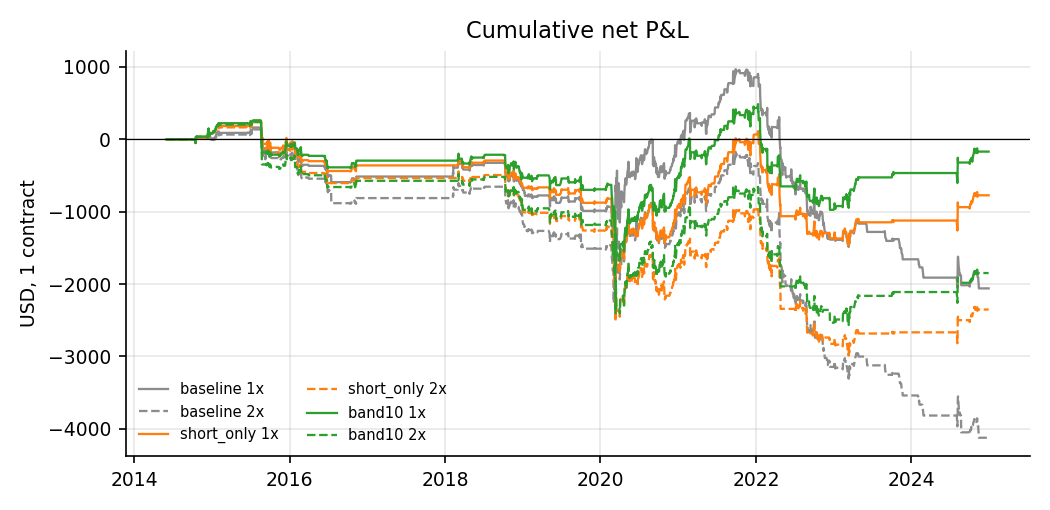
\includegraphics[width=0.92\linewidth]{figures/cum_pnl.png}\caption{Cumulative net P\&L, 1x solid and 2x dashed; baseline (live rules) grey}\end{figure}

\texttt{band10} and \texttt{short\_\allowbreak{}only} stay close until 2018, then \texttt{band10} pulls ahead slowly through 2019-2020 and again in 2023. Both books fall the same way in the March 2020 sell-off and in 2022. The gap at the end is \$603 at 1x and \$504 at 2x.

\begin{figure}[H]\centering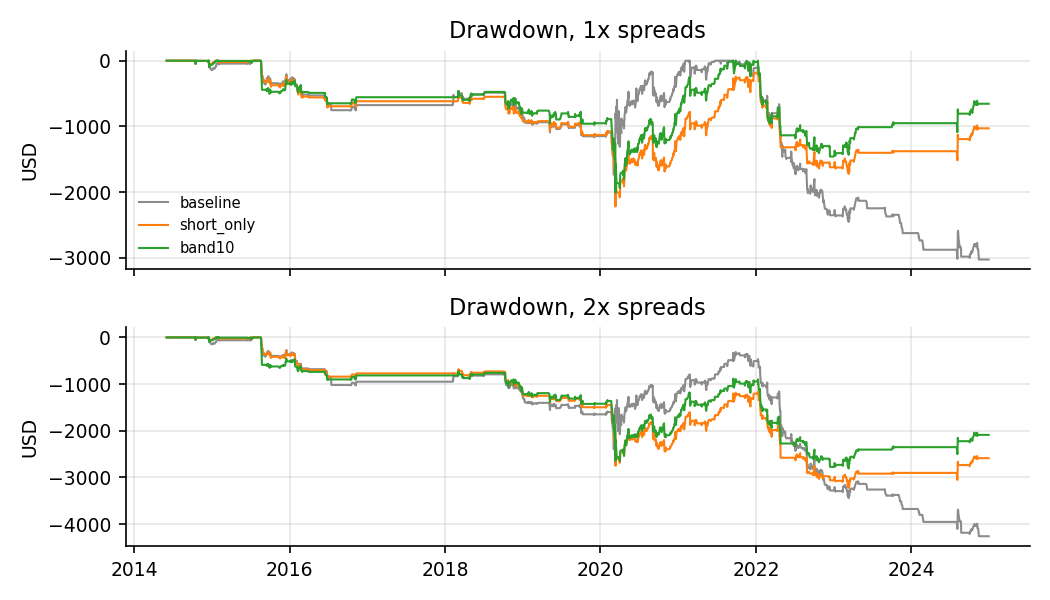
\includegraphics[width=0.92\linewidth]{figures/drawdown.png}\caption{Drawdown at 1x and 2x spreads}\end{figure}

The worst drawdown has the same trough date in both books: 2020-03-12 at 1x and 2023-03-13 at 2x. \texttt{band10} is shallower in both, \$2,010 against \$2,220 at 1x and \$2,806 against \$3,222 at 2x.

\begin{figure}[H]\centering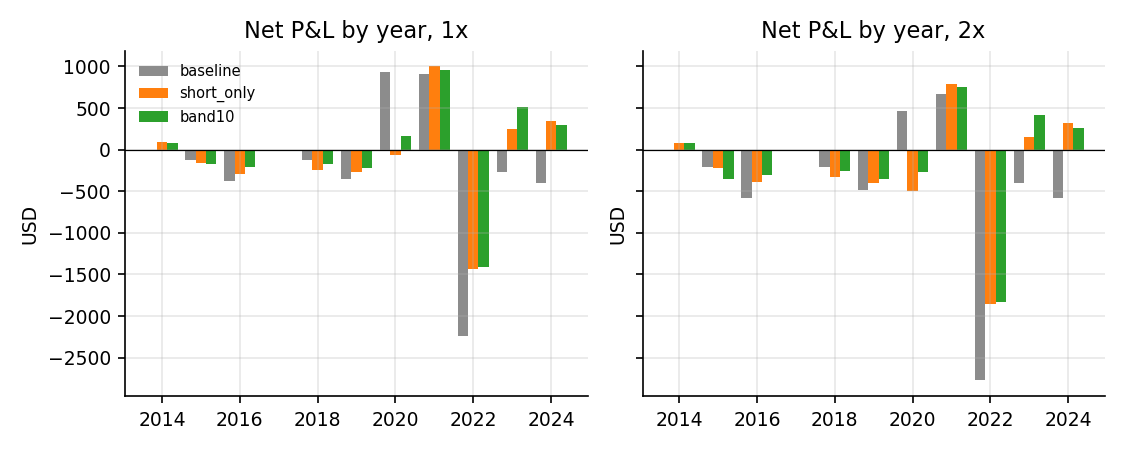
\includegraphics[width=0.92\linewidth]{figures/yearly.png}\caption{Net P\&L by year}\end{figure}

At 1x, \texttt{band10} is ahead in 6 of the 10 years that have trades (2017 has none): 2016 (+\$87), 2018 (+\$72), 2019 (+\$47), 2020 (+\$219), 2022 (+\$27) and 2023 (+\$264). It is behind in 2014 (\ensuremath{-}\$2), 2015 (\ensuremath{-}\$19), 2021 (\ensuremath{-}\$38) and 2024 (\ensuremath{-}\$53). At 2x, 2015 is worse (\ensuremath{-}\$124) because of one stop, discussed below. 2020 and 2023 give \$483 of the \$603 gain at 1x.

\begin{figure}[H]\centering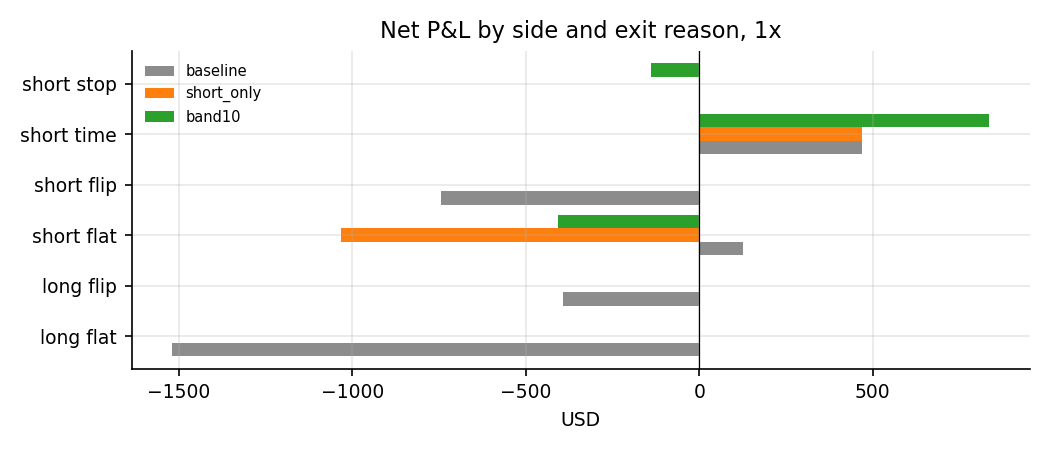
\includegraphics[width=0.92\linewidth]{figures/by_reason.png}\caption{Net P\&L by side and exit reason, 1x}\end{figure}

Both books close the same 13 shorts at the 7-DTE time exit. With the band, those 13 make \$835 net instead of \$470. The flat-exit shorts lose \$407 instead of \$1,032. One short that \texttt{short\_\allowbreak{}only} closed on a flat signal hits the stop under \texttt{band10} instead (the only stop in either book).

\begin{figure}[H]\centering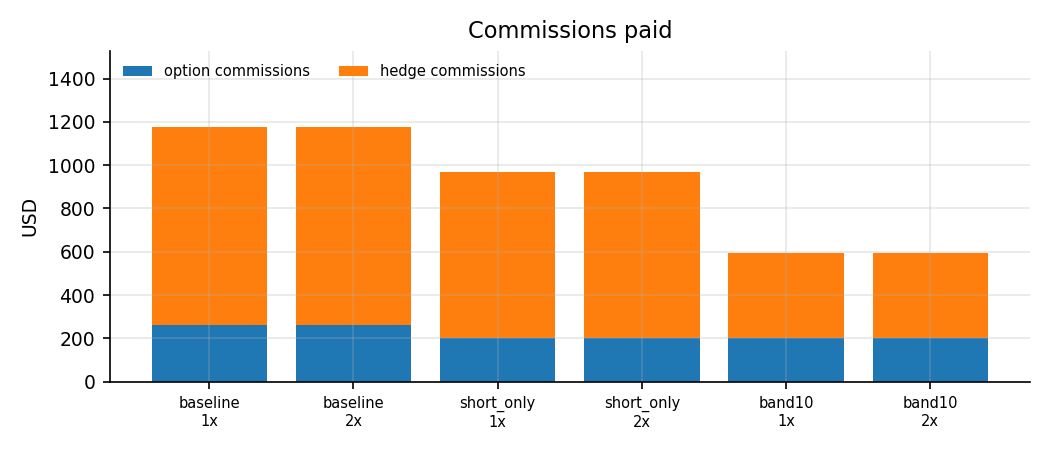
\includegraphics[width=0.92\linewidth]{figures/fees.png}\caption{Commissions paid}\end{figure}

Option commissions are the same (\$200, 100 round trips). Hedge commissions fall from \$770 to \$395. With 1 contract every hedge order costs the \$1 minimum, so hedge commissions equal the number of hedge orders.

\begin{figure}[H]\centering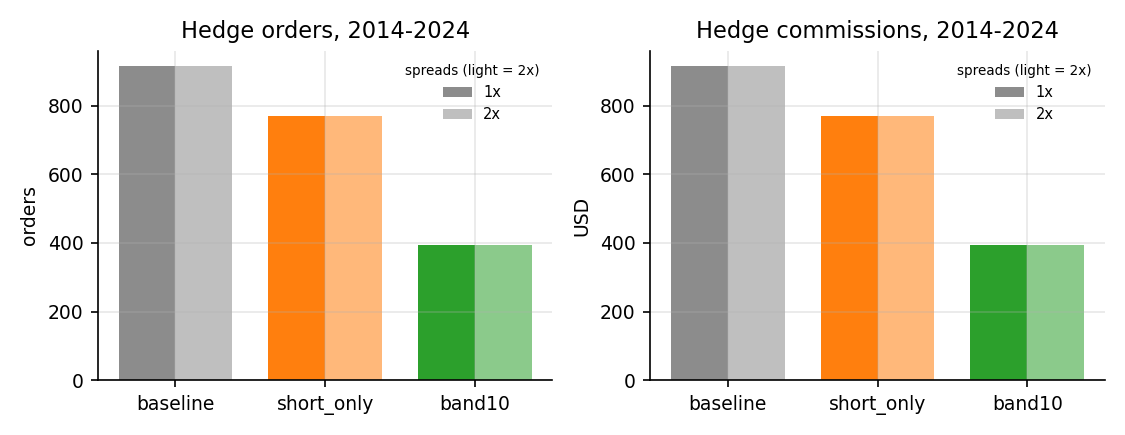
\includegraphics[width=0.92\linewidth]{figures/hedging.png}\caption{Hedge orders and hedge commissions, 2014-2024; darker 1x, lighter 2x}\end{figure}

The band cuts hedge orders by 49\%, from 770 to 395. That clears the 20\% event floor easily, and it is the same cut the band made on the baseline book (914 to 469). The spread multiple doesn't change hedging: the 1x and 2x hedge orders are identical.

\begin{figure}[H]\centering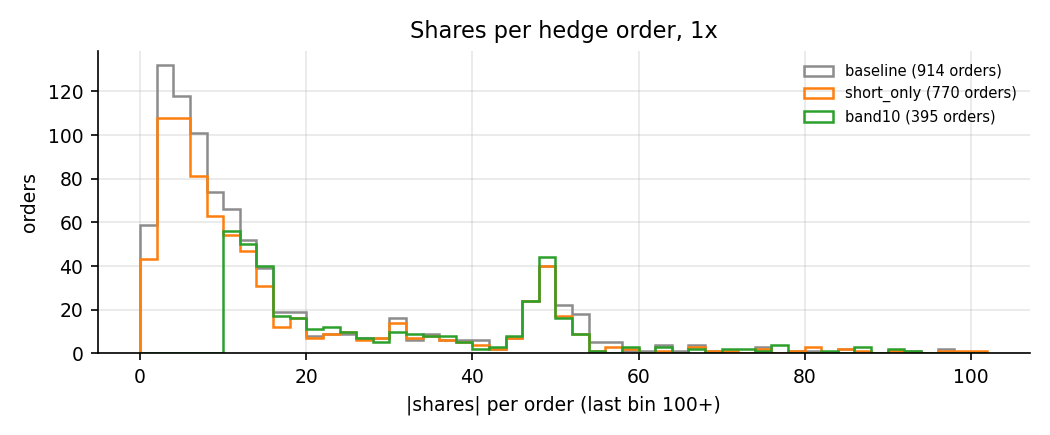
\includegraphics[width=0.92\linewidth]{figures/hedge_sizes.png}\caption{Shares per hedge order, 1x}\end{figure}

Without the band, 403 of the 770 short-only hedge orders (52\%) are for fewer than 10 shares. The median order is 9 shares. With the band no order is under 10 shares, and the median is 23. Above 10 shares the two histograms are almost the same, so the band removes the small orders and leaves the rest alone.

\begin{figure}[H]\centering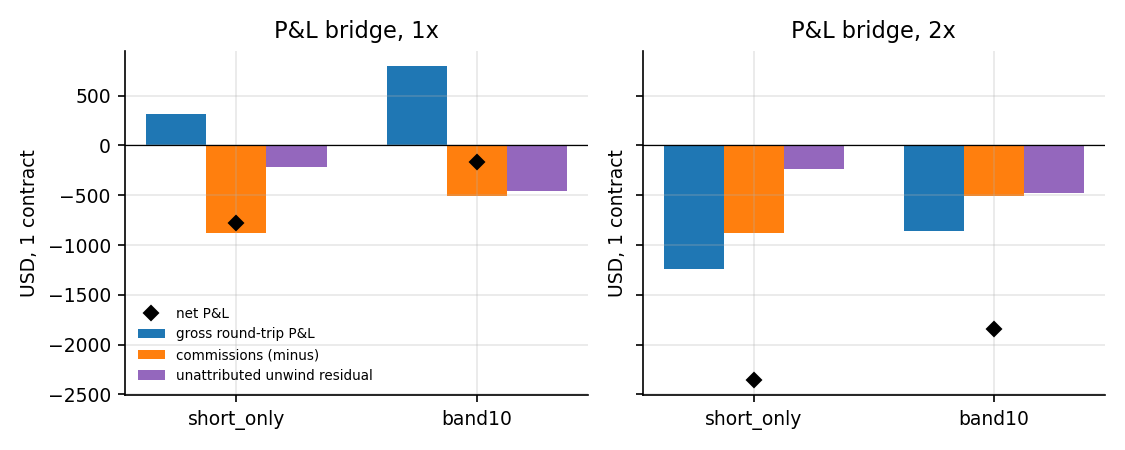
\includegraphics[width=0.92\linewidth]{figures/pnl_bridge.png}\caption{P\&L bridge: gross round-trip P\&L, commissions and the unattributed unwind residual}\end{figure}

Net P\&L is gross round-trip P\&L, minus the commissions attributed to round trips, plus a residual. The residual is equity minus round-trip net P\&L. Most of it is hedge-unwind fill gaps: a round trip values its shares at the 10:15 decision spot, but the unwind order fills in the next 15 minutes. The table below gives the bridge of the change.

\begin{center}\small
\begin{tabularx}{\linewidth}{>{\raggedright\arraybackslash}X l l}
\toprule
\textbf{Change, band10 minus short\_only} & \textbf{1x} & \textbf{2x} \\
\midrule
Gross round-trip P\&L & +477 & +378 \\
Commissions attributed to round trips (saved) & +375 & +375 \\
Unattributed unwind residual & \ensuremath{-}248 & \ensuremath{-}249 \\
\textbf{Net P\&L} & \textbf{+603} & \textbf{+504} \\
\bottomrule
\end{tabularx}
\end{center}

\section{Analysis}

\textbf{The fee saving is mechanical.} The band removes 375 hedge orders, and each one cost the \$1 minimum, so \$375 is saved at both spreads. That is 62\% of the gain at 1x and 74\% at 2x. The 90 unwind orders after closes cost the same \$90 in both books and sit in the residual.

\textbf{The gross gain is mostly path P\&L and may be noise.} 99 of the 100 round trips have the same entry, exit date and exit reason in both books. On those 99, the band adds \$361 gross at 1x (+\$368 at 2x). The gain is spread out: 47 trips gain, 49 lose, the median change is zero, and the five largest changes are 22\% of the total absolute change. The 13 time-exit trips, held longest, give \$254 of the \$361. Smaller fill gaps on in-position hedge orders are worth only about \$39 across all trades (the band trades fewer, larger orders). The rest is the share leg following a different path. The same thing happened on the baseline book, where the band's share-leg gain was not steady across band sizes. So the gross gain should not be expected to repeat at this size.

\textbf{One changed trade: the 2015-08-24 stop.} The 100th round trip is a short opened in August 2015. Under \texttt{short\_\allowbreak{}only} it closed on a flat signal on 2015-08-27, losing \$250 gross. Under \texttt{band10} its option-plus-hedge P\&L crossed the stop at 10:15 on 2015-08-24, the morning of the flash crash, and it closed for \ensuremath{-}\$134 gross (+\$116 at 1x). The 73-share unwind then filled about \$4.16 a share away from the decision spot, which cost \$303. That one order is almost all of the \ensuremath{-}\$248 change in the residual. Without that day the residual change is +\$55. The stop is the same event that appeared in the hedge-band study: the band lets a short's hedge drift further, so stops can fire where they didn't before. At 2x the stop close also pays a wider option spread, so 2015 costs \$124 at 2x against \$19 at 1x.

\textbf{Do the rules add up?} Short-only gained \$1,286 at 1x over the baseline, and the band gained \$963 on the baseline book. Together they gain \$1,889, which is 84\% of the sum of the two separate gains (86\% at 2x). The band is worth less on the short-only book (\$603 against \$963 at 1x) for two reasons. There are fewer orders to remove (375 against 445). The 2015 stop also lands on this book.

\section{Verdict}

\textbf{Passed} on the pre-registered bar, at 1x and 2x, in both halves, with the tail guard and the event floor met. The 2014-2019 margin is thin at 2x (\$81), and over half of the full-window gain at 1x (\$361 of \$603) is share-path P\&L on matched trades that may be noise. The mechanical part, \$375 of hedge commissions saved, holds at both spreads. The next step, if the PM approves, is one hold-out run of \texttt{band10} against the hold-out baseline (2025-01-01 to 2026-07-10) on the card's hold-out bar. After that come shadow mode, a decision record and the two-line \texttt{paper.\allowbreak{}toml} change.

\section{Caveats}

\begin{itemize}

\item \textbf{In-sample:} the idea comes from the 2026-10-16 desk discussion of the baseline and from the short-only and hedge-band results, all on this same window. Only the hold-out can confirm it.

\item \textbf{One contract:} the \$1 minimum per order is large relative to size. With more contracts each hedge order is bigger, so the fee saving per contract shrinks.

\item \textbf{Spread model:} fitted on about two weeks of calm 2026 live quotes; the 2x run is the stress test.

\item \textbf{Data gaps:} R2 has no month-end weekdays, so about 3.3\% of scheduled times are skipped (89 at each spread).

\item \textbf{Few events:} the band fired throughout (395 orders instead of 770), but the result rests on 100 round trips, 38 of them in the first half. One stop on a crash morning moves the residual by \$303.

\item \textbf{Fill timing:} hedge and unwind orders fill on trades in the 15 minutes after the decision. On fast days this gap is a few dollars a share, and it is mostly noise from that timing rule.

\item \textbf{Reused reference:} \texttt{short\_\allowbreak{}only} was not rerun here. Its saved config matches \texttt{band10} except \texttt{min\_\allowbreak{}shares}, and an identical config rerun under \texttt{2026-\allowbreak{}10-\allowbreak{}16-\allowbreak{}no-\allowbreak{}flat-\allowbreak{}exit} (after the latest engine change) reproduced its equity exactly.

\end{itemize}

\section{Trials}

2 trials for this experiment (\texttt{band10} at 1x and 2x, one run of \texttt{experiment.\allowbreak{}py} at commit c2f7109, not dirty). The reference was reused from \texttt{2026-\allowbreak{}10-\allowbreak{}16-\allowbreak{}short-\allowbreak{}only} (2 trials, not rerun), and baseline trial 1 (2 trials) is shown for context. The pass bar was not changed.

\end{document}
